% This is samplepaper.tex, a sample chapter demonstrating the
% LLNCS macro package for Springer Computer Science proceedings;
% Version 2.21 of 2022/01/12
%
\documentclass[runningheads]{llncs}
%
\usepackage[T1]{fontenc}
% T1 fonts will be used to generate the final print and online PDFs,
% so please use T1 fonts in your manuscript whenever possible.
% Other font encondings may result in incorrect characters.
%
\usepackage{graphicx}
% Used for displaying a sample figure. If possible, figure files should
% be included in EPS format.
%
% If you use the hyperref package, please uncomment the following two lines
% to display URLs in blue roman font according to Springer's eBook style:
%\usepackage{color}
%\renewcommand\UrlFont{\color{blue}\rmfamily}
%\urlstyle{rm}
\usepackage{hyperref}
\usepackage[acronym]{glossaries}
\glsdisablehyper
\usepackage{todonotes}
\usepackage{subcaption}
\usepackage{caption}
\captionsetup[table]{name=Tab.}
\usepackage{xspace}
\usepackage{siunitx}
\usepackage{multicol}
\usepackage{multirow}
\usepackage{booktabs}
\usepackage{svg}
\usepackage{xurl}
\usepackage[sort,compress]{cite}

% \usepackage{draftwatermark}
% \SetWatermarkText{DRAFT}
% \SetWatermarkScale{5}
% \usepackage{framed}

% I inserted this since I always got a numbered but blank first page
% I do not know why
% I followed this advise: https://tex.stackexchange.com/a/434340
\usepackage{atbegshi}
\AtBeginDocument{\AtBeginShipoutNext{\AtBeginShipoutDiscard}\addtocounter{page}{-1}}



\newcommand{\citeurl}[1]{\unskip\footnote{{\scriptsize \url{#1}}}}
\newcommand{\pkgname}[1]{{\scriptsize \textsf{#1}}}
\newcommand{\projname}[1]{{\small \textsf{#1}}}
% \newcommand{\toolname}[1]{{\scriptsize \texttt{#1}}}
\newcommand{\toolname}[1]{{\small \texttt{#1}}}

\newcommand{\python}{\projname{Python}\xspace}
\newcommand{\cp}{\projname{CPython}\xspace}
\newcommand{\cpv}[1]{\projname{CPython 3.{#1}}\xspace}
\newcommand{\flask}{\projname{Flask}\xspace}
\newcommand{\django}{\projname{Django}\xspace}
\newcommand{\rust}{\projname{Rust}\xspace}
\newcommand{\java}{\projname{Java}\xspace}
\newcommand{\cc}{\projname{C\nolinebreak\hspace{-.05em}\raisebox{.4ex}{\tiny +}\nolinebreak\hspace{-.10em}\raisebox{.4ex}{\tiny +}}\xspace}

\renewcommand{\tableautorefname}{Tab.}
\renewcommand{\figureautorefname}{Fig.}
\renewcommand{\sectionautorefname}{Sec.}
\renewcommand{\subsectionautorefname}{Sec.}
\renewcommand{\subsubsectionautorefname}{Sec.}

\newacronym{pep}{PEP}{Python Enhancement Proposal}
\newacronym{watt}{W}{Watt}
\newacronym{joule}{J}{Joule}
\newacronym{sut}{SUT}{System Under Test}
\newacronym{pypi}{PyPI}{Python Packaging Index}
\newacronym{pyperformance}{\projname{pyperformance}}{The Python Performance Benchmark Suite}
\newacronym{os}{OS}{Operating System}
\newacronym{cpu}{CPU}{Central Processing Unit}
\newacronym{rpi}{RPI}{Raspberry Pi}
\newacronym{rapl}{RAPL}{Running Average Power Limit}


\newcommand{\rpi}[1]{\toolname{Raspberri Pi #1}\xspace}
\newcommand{\rpia}{\gls{rpi}\xspace}

%
% Page limit: 12 to 16 pages
\begin{document}
%
\title{Energy Consumption of Python Performance Benchmarks Depends on Execution Environments}
%
%\titlerunning{Abbreviated paper title}
% If the paper title is too long for the running head, you can set
% an abbreviated paper title here
%
\author{Oskar Emil Breindahl\inst{1}
\and
Rolf-Helge Pfeiffer\inst{1}\orcidID{0000-0003-2585-6473}
%\and
%Third Author\inst{3}\orcidID{2222--3333-4444-5555}
}
%
\authorrunning{O. Breindahl, R.-H. Pfeiffer}\
\titlerunning{Energy Consumption Depends on Execution Environments}
%\authorrunning{Fst. Author}\
% First names are abbreviated in the running head.
% If there are more than two authors, 'et al.' is used.
%
\institute{IT University of Copenhagen, Rued Langgaards Vej 7, 2300 Copenhagen
\email{\{osbr,ropf\}@itu.dk}}
% \institute{A University, Street, City
% \email{author@university.edu}}
%\url{http://www.springer.com/gp/computer-science/lncs} \and
%ABC Institute, Rupert-Karls-University Heidelberg, Heidelberg, Germany\\
%\email{\{abc,lncs\}@uni-heidelberg.de}}
%
\maketitle              % typeset the header of the contribution
%
\begin{abstract}
% The abstract should briefly summarize the contents of the paper in 150--250 words.
\python is one of the most used programming languages in the world.
Developers of the \python interpreter increase its performance over recent releases and measure these with \gls{pyperformance}.
However, little is known about the impact of performance increases on the energy consumption of \python programs when executed in different environments like operating systems or processors.
In this paper, we study via a controlled lab experiment the energy consumption of benchmarks from \gls{pyperformance} when executed on five versions of the \python interpreter \cp, on four different operating systems, and on two different processors.
Our results indicate that executing Python programs on a Cortex-A72 processor running Manjaro Linux and \cpv{12} is XX times more energy efficient than on a Cortex-A53 running FreeBSD with \cpv{10}.
Even on the same processor, energy consumption of \python programs decreases by up to XX\% when executed on Manjaro Linux and a newer versions of \python, compared to other operating systems and older versions of \cp.
\keywords{Software engineering \and Energy consumption \and CPython.}
\end{abstract}

\section{Introduction}\label{sec:introduction}

The responsibility of software developers to create sustainable and energy-efficient software is becoming more and more apparent\cite{caballar2024we} and the environmental impact and sustainability of software is increasingly studied.\cite{ahmad2023green,caballar2024we,freed2023investigation,gupta2021chasing,adersma2022green,lamprakos_energy,holm2020gpu,reya2023greenpy,lorincz2019greener,freed2023investigation,roque2025unveiling,paul2023comprehensive,ahmad2023green,tiwari2021review}\todo{Too much sausage?}.

\python is likely the most popular~\cite{djurdjev2024popularity,pypl,tiobe} and most used~\cite{stackover, statista} programming language in the world.
Big corporations create software products with it.
For example, Google’s \projname{YouTube} is powered by \python~\cite{winters2020software}, circa 20\% of \projname{Facebook}’s infrastructure is written in \python~\cite{komorn2016python}, \projname{Instagram} is a \python application~\cite{ni2016web}, or circa 80\% of \projname{Spotify}’s backend services are written in \python~\cite{van2013how}.

Like other dynamically typed and interpreted programming languages, running certain \python programs is reported to be slow and of low energy efficiency~\cite{pereira_rank_efficiency}.
In recent years, the developers of \cp, the reference implementation of the \python interpreter, continuously increase the performance of \cp, i.e., they increase execution times of \python programs.

Since energy consumption of software is influenced by execution times ($E = P \times t$) and since \python is a comparably slow dynamically typed interpreted language, it might be worthwhile to continue to increase performance of \cp over the coming releases.
We believe that additionally focusing on the energy consumption of programs executed on \cp should be in focus as well.\todo{Improve this.}
Currently, there is no \gls{pep} to reduce energy consumption of \python programs as there are \glspl{pep} to increase performance of \cp~\cite{pep_index}.

In this paper, we present a light weight experiment design that allows to compare the energy consumption of \python programs that are executed on various configurations of hardware, \gls{os}, and \python versions.
Our goals are \emph{a)} to investigate if certain configurations of \glspl{cpu}, \glspl{os}, and \python versions significantly impact the energy consumption of \python benchmarks from \gls{pyperformance}, and \emph{b)} to provide an experiment design that is so light weight that \cp developers can efficiently include it in their current setup when running \gls{pyperformance}.

We investigate the following three research questions:
\begin{itemize}
  \item \textbf{RQ1:} \textit{How do different \glspl{cpu} impact the energy consumption of \gls{pyperformance} benchmarks?}
  \item \textbf{RQ2:} \textit{How do different \glspl{os} impact the energy consumption of \gls{pyperformance} benchmarks?}
  \item \textbf{RQ3:} \textit{How do different versions of \cp impact the energy consumption of \gls{pyperformance} benchmarks?}
\end{itemize}

We measure energy consumption of a \gls{sut} with an \toolname{Otii Ace Pro}~\cite{qoitech2022otii}.
In this paper, \glspl{sut} are a \toolname{Raspberry Pi 3B+} (ARM-Cortex-A53) and \toolname{Raspberry Pi 4B} (ARM-Cortex A72) respectively.
% TODO: Add these to references
% https://datasheets.raspberrypi.com/rpi3/raspberry-pi-3-b-plus-product-brief.pdf
% https://datasheets.raspberrypi.com/rpi4/raspberry-pi-4-datasheet.pdf
On each \toolname{Raspberry Pi}, we sequentially deploy one of the four Unix(-like) \glspl{os} \projname{Alpine}, \projname{Manjaro}, \projname{Ubuntu}, and \projname{FreeBSD}.
On each \gls{os}, we sequentially deploy different versions of \cp.
The combination of \gls{cpu}, \gls{os}, and version of \cp is a configuration.
In our experiment, we investigate 40 different configurations.
For each configuration, we execute \gls{pyperformance} and measure execution times of various benchmarks and their power draw during execution.

We find that all three variables of \gls{cpu}, \gls{os}, and version of \cp have a statistically significant impact on energy consumption during benchmark execution.
\todo{Fill in high level results here once the paper is stable}
% Fill in high level results here!


The contributions of this paper are:
\begin{itemize}
  \item We present an experiment design to directly measure the energy consumption of 40 different configurations of \gls{cpu}, \gls{os}, and version of \cp.
  \item We demonstrate that benchmarks executed on certain configurations of \gls{cpu}, \gls{os}, and version of \cp consume significantly less energy compared to other widely used configurations.
  \item We provide a replication kit\footnote{\url{https://github.com/oskarbreindahl/Python_Application_Energy_Consumption}} that allows to automatically replicate our results. It also contains all results reported in this paper and allows for reproduction.\todo{Move repo and anonymize link for review.}
\end{itemize}

\section{Background \& Terminology}\label{sec:background}

\noindent\textbf{System Under Test:} \emph{Raspberry Pis} are credit card sized ARM-based single-board computers produced by the Raspberry Pi Foundation\cite{raspberry_pi_website}.
These inexpensive computers are often used in lab experiments, e.g., \cite{zhao2015exploring,pfeiffer2024energy}.\todo{Check if the former can be used for that statement.}
We use two versions of \toolname{Raspberry Pis} as \glspl{sut} for the research in this paper.
First, the \toolname{Raspberry Pi 3B+} with a four core ARM-Cortex-A53 \gls{cpu} and 1GB RAM and second, the \toolname{Raspberry Pi 4B} with a four core ARM-Cortex A72 \gls{cpu} and XXGB RAM\todo{Which version did you use?}.
Both processors are 64-bit running at 1.4GHz and 1.8GHz respectively.
The main difference between the Cortex-A53 and A72 architecture is that the latter supports out-of-order memory operations.

\noindent\textbf{Operating Systems:} We execute our experiment on four \glspl{os}.
One Unix, \projname{FreeBSD}\cite{freebsd_website}, and the three Linux distributions \projname{Alpine}\cite{alpine_website}, \projname{Manjaro}\cite{manjaro_website} and \projname{Ubuntu}\cite{ubuntu_website}.\todo{Add precise versions+kernel and libc versions}
In the Linux realm, \emph{distributions} are a collection of \gls{os} kernel, init system, tools, and applications, which in the case of Unixes like \projname{FreeBSD} are all provided together as a single system.
For example, \projname{Ubuntu} is a \projname{Debian}-based distribution (relying on \projname{systemd} and the \projname{apt} package manager) that focuses on stability and \projname{Manjaro} is based on \projname{Arch Linux} (relying on \projname{systemd} and the \projname{pacman} package manager) with a rolling-release update model.
\projname{Alpine Linux} differs from the other two Linuxes in the choice of basic software.
It relies on \projname{musl} instead of \projname{glibc} as C standard library, \projname{BusyBox} instead of \projname{GNU Core Utilities}, and \projname{OpenRC} as init system instead of \projname{systemd}.
\todo{Add sentence on popularity and widely used on servers/containers}

\noindent\textbf{Python:} is likely the most popular~\cite{djurdjev2024popularity,pypl,tiobe} and most used~\cite{stackover, statista} programming language in the world.
There are many different implementations of the language, e.g., the reference implementation \cp, \projname{pypy}, \projname{MicroPython}, etc.
In this paper we consider the --at the time of writing-- latest releases of the five supported versions of \cp: \cpv{9.22}, \cpv{10.17}, \cpv{11.12}, \cpv{12.10}, and \cpv{13.3}.
In the remainder, we denote these versions by their major and minor version number, e.g., \cpv{9}, \cpv{10}, etc.

\noindent\textbf{\acrlong{pyperformance}:} is an open-source benchmarking tool~\cite{pyperf_git} that \cp developers use to report performance improvements of new versions of \cp, see e.g., the release notes for \cpv{12}~\cite{py312}.
\gls{pyperformance} consists of 87 benchmark programs that are organized in seven \emph{groups}.
For our experiment, we select three \textit{``'High-level' applicative benchmarks''}\cite{pyperf_docs} benchmarks from the \toolname{apps} group: \toolname{2to3}, \toolname{tornado\_http} and \toolname{chameleon}.


\noindent\textbf{Measuring Energy Consumption:} There are two main ways to measure the energy consumption of a \gls{sut}.
On certain Intel-based processors, one could use \gls{rapl}~\cite{khan2018rapl}, which is a built-in \gls{cpu} feature that allows --amongst others-- to estimate power draw of running programs.
% https://greencompute.uk/Measurement/RAPL
Since this feature is not available on a broad range of \glspl{cpu}, e.g., the ARM-Cortex architectures in our experiment, one can always directly measure power draw of a \gls{sut} with a suitable power meter~\cite{kavanagh2019rapid}.
In our experiment, we use the \toolname{Otii Ace Pro}~\cite{otii_website,qoitech2022otii}, which is a power supply with combined scriptable power-meter.
We use it to record \emph{power draw} ($P$ in Watts [W]) and execution times of benchmarks (in seconds [s])
We compute \emph{energy consumption} ($E$ in Joules [J]) via $E = P \times t$.
\section{Experiment Design}\label{sec:experimentdesign}

\begin{figure}[t]
\begin{subfigure}[t]{0.58\textwidth}
    \centering
    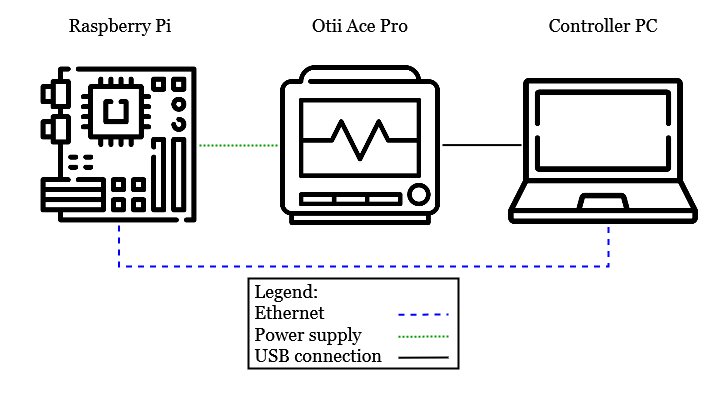
\includegraphics[width=\textwidth]{images/experiment.png}
    \caption{Experiment design for measuring power draw and runtime of \gls{sut} while executing \gls{pyperformance} benchmarks.}
    \label{fig:design}
\end{subfigure}
\hspace{\fill}
\begin{subfigure}[t]{0.4\textwidth}
    \centering
    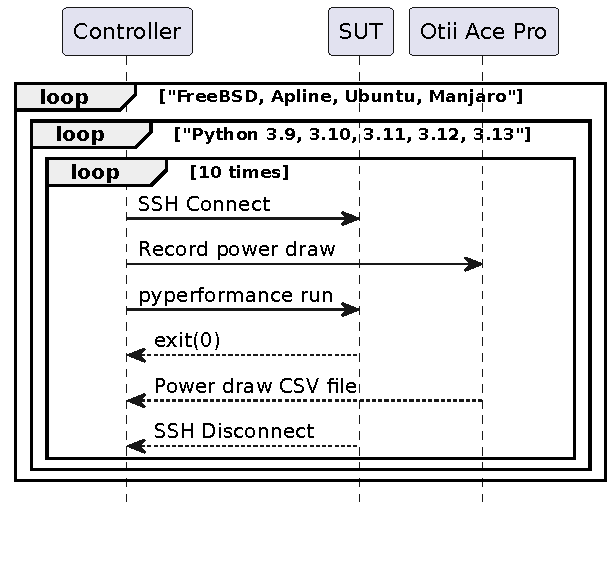
\includegraphics[width=\textwidth]{images/scenario.pdf}
    \caption{Interactions between the controller computer initiating power draw recordings and benchmark executions.}
    \label{fig:sequence}
\end{subfigure}
\caption{Illustration of our experiment design.}\label{fig:exp_scen}
\end{figure}





\autoref{fig:design} illustrates our experiment design.
The \toolname{Otii Arc Pro} in the center, powers a \toolname{Raspberry Pi} (\gls{sut}) via USB-C.
At the same time, it serves as a power meter recording the power draw of the \gls{sut} (illustrated by a green line).
A controller computer (to the right in \autoref{fig:design}) is connected via USB to the power meter (black line).
Using the \toolname{Otii 3 Desktop App}
% https://docs.qoitech.com/user-manual/otii/software/otii3-desktop-app
and the \toolname{Otii Automation Toolbox}
% https://www.qoitech.com/automation-toolbox/
, the controller computer can trigger a measurement and collect all power meter recordings automatically.

Both the \gls{sut} and the controller computer are connected via ethernet to a local network (blue line).
By that connection, the controller computer initiates executions of \acrlong{pyperformance} on the \gls{sut}.

Not illustrated in \autoref{fig:design} is a 25V lab power supply powering the \toolname{Otii Arc Pro} and a room fan that is placed next to the \gls{sut} to keep \gls{cpu} temperature on a constant level.

Prior to the experiment, we prepare four SD-cards.
One with \projname{FreeBSD}, \projname{Alpine}, \projname{Manjaro}, and \projname{Ubuntu} Linux respectively\todo{Add precise versions+kernel and libc versions}, see our replication kit for details.
On each of these, we automatically install the five versions of \python (\cpv{9} to \cpv{13}) from source together with the \gls{pyperformance} tool.\todo{Did that include tuning?}
Each operating system and each version of \python is setup in default configuration.



% A large fan is set up to continually cool the RPi, and CPU temperature is then queried directly on the RPi through another SSH terminal on the PC, before, during, and after benchmarks.
% This is to make sure that rising CPU temperature doesn't skew the measurements for longer benchmarks, since CPUs are known to perform worse at higher temperatures\cite{benoit2020impact}.
% TODO: Move that to Threats
% Throughout the entire benchmarking process, the CPU temperature never rises above 37$^{\circ}$C, which is deemed satisfactory for consistency of results.
% OSs are installed in their default configurations to make sure that any potential differences in energy consumption between them can be explained by the OS implementation specifics alone, and not by the quality of performance optimizations made by the user.

Per configuration of \gls{cpu}, \gls{os}, and version of \python, we execute the \gls{pyperformance} benchmarks ten times\todo{@oskar: you experiment script does it 11 times, why?} and record power draw for each invocation of the benchmarks, see the inner most loop in\autoref{fig:sequence}.
Note, per default, \gls{pyperformance} executes each benchmark ten times per invocation of the tool.\todo{Double check that! I believe it is more often.}
We omit to illustrate this internal behavior in \autoref{fig:sequence} and consider \gls{pyperformance} as a black box in our experiment.
The ten invocations of the \gls{pyperformance} benchmarks is repeated five times, i.e., on each version of \python (\cpv{9} to \cpv{13}), see nested loop on level two in \autoref{fig:sequence}.
These two steps of the experiment are automated via scripts.
The benchmarks are invoked 10 times per version of \python on each of the four \gls{os}, \projname{FreeBSD}, \projname{Alpine}, \projname{Manjaro}, and \projname{Ubuntu} Linux, see outer most loop in \autoref{fig:sequence}, and in turn on each of the two \gls{sut} (\toolname{Raspberry Pi 3B+} and \toolname{4B} respectively.
These latter two experiment steps are manual since they require to power-down the respective \gls{sut} and replace the SD-card or to replace the \gls{sut} (not illustrated in \autoref{fig:sequence}).

In total, we collect 400 measurements, i.e., 10 invocations of \gls{pyperformance} on five versions of \python on four \gls{os} on two \gls{sut}.
All collected measurements are automatically stored in CSV files, which we aggregate for further analysis for the following sections.
\section{Results}\label{sec:results}

% Each recording made with the Otii software samples power draw in watts 10,000 times per second. For every unique configuration of RPi, OS, and Python version, 10 recordings are made -- one for each benchmarking run. Average power draw and the runtime in seconds are extracted from each individual recording, with energy consumption in joules being calculated immediately as well. These results are then written to a CSV file uniquely named by the three parameters, e.g. \texttt{results\_RPi3B+\_Alpine\_python3.9.csv}, such that every CSV file contains the results for the 10 recordings made for that configuration. The CSV files can all be found in the repository.



\begin{figure}[t]
    \centering
    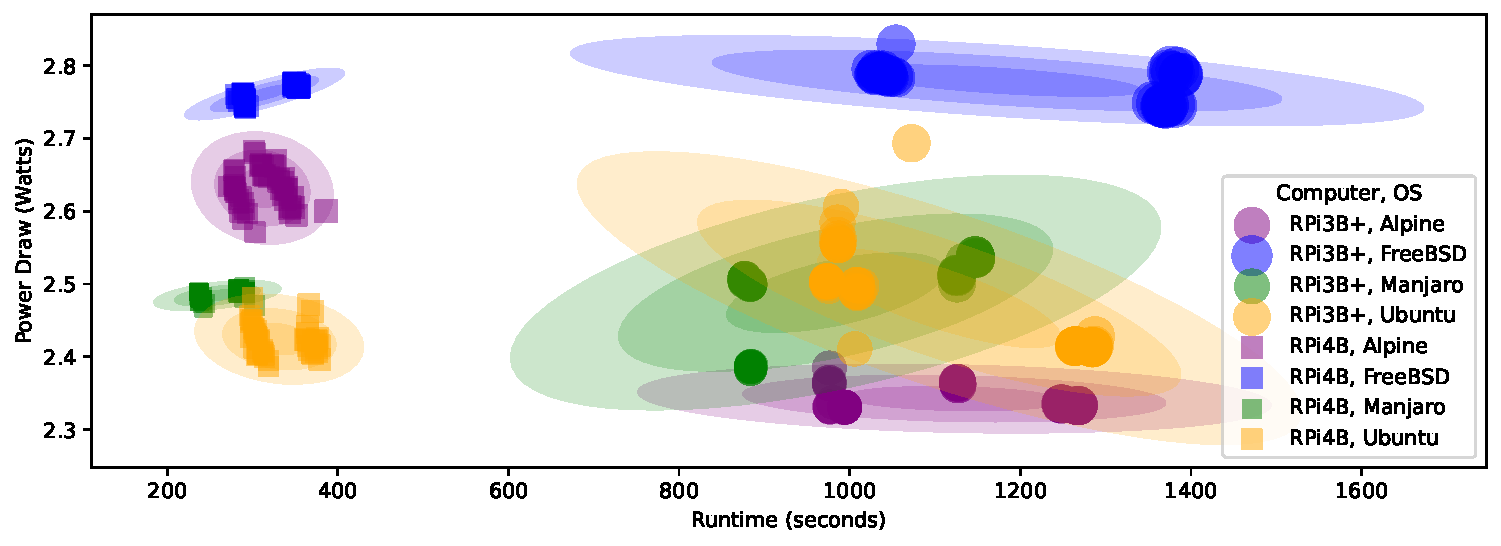
\includegraphics[width=1\textwidth]{images/P_t_E_bagplot.pdf}
    \caption{.}
    \label{fig:results}
\end{figure}

\autoref{fig:results} illustrates the results of our measurements as a scatter plot.
The x-axis shows the runtime of a \gls{pyperformance} benchmark in seconds.
The y-axis lists the measured power draw in Watts.
Each element in the scatter plot corresponds to the power draw and runtime of a benchmark in a certain configuration.
Shapes of elements (squares to the left and circles to the right) denote the \gls{sut} on which a benchmark is executed.
Color of elements corresponds to the respective \gls{os}.
The size of each element is proportional to the energy consumption of a benchmark execution, i.e., the product of power draw and runtime.


Note, for reporting we use the following notation:
$q_{0}$ denotes the minimum,
$q_{1}$ the 25\textsuperscript{th} quartile,
$q_{2}$ the median,
$q_{3}$ the 75\textsuperscript{th} quartile,
$q_{4}$ the maximum,
$\mu$ is the arithmetic mean (we use average and arithmetic mean synonymously),
and the standard deviation is denoted by $\sigma$.

It can be seen that benchmarks run faster on the \toolname{Raspberry Pi 4B}
($q_{0} \approx 237.13\unit{\second}$,
$q_{1} \approx 283.86\unit{\second}$,
$q_{2} \approx 297.51\unit{\second}$,
$q_{3} \approx 338.6\unit{\second}$,
$q_{4} \approx 386.52\unit{\second}$,
$\mu \approx 303.95\unit{\second}$,
$\sigma \approx39.66$)
compared to a \toolname{Raspberry Pi 3B+}
($q_{0} \approx 876.03\unit{\second}$,
$q_{1} \approx 984.18\unit{\second}$,
$q_{2} \approx 1042.14\unit{\second}$,
$q_{3} \approx 1253.09\unit{\second}$,
$q_{4} \approx 1388.55\unit{\second}$,
$\mu \approx 1096.04\unit{\second}$,
$\sigma \approx 155.79$).
The longest runtime ($23\unit{\minute}:08\unit{\second}$) of a benchmark is on a \toolname{Raspberry Pi 3B+} with \projname{FreeBSD} and \cpv{10} whereas the fastest ($3\unit{\minute}:57\unit{\second}$) is on a \toolname{Raspberry Pi 4B} with \projname{Manjaro} and \cpv{11}.

Power draw of benchmark execution in any configuration varies in the range of $500mW$
($q_{0} \approx 2.33\unit{\watt}$,
$q_{1} \approx 2.42\unit{\watt}$,
$q_{2} \approx 2.50\unit{\watt}$,
$q_{3} \approx 2.71\unit{\watt}$,
$q_{4} \approx 2.83\unit{\watt}$,
$\mu \approx 2.55\unit{\watt}$,
$\sigma \approx 0.15$).
The highest power draw of a benchmark is on a \toolname{Raspberry Pi 3B+} with \projname{FreeBSD} and \cpv{13} and the lowest is on a \toolname{Raspberry Pi 3B+} with \projname{Alpine} and \cpv{11}.
\todo{Explain bags}

To facilitate statistical analysis and visual inspection, we illustrate and discuss the energy consumptions of the \gls{pyperformance} benchmarks separately over \gls{sut}, \gls{os}, and version pf \python, see \autoref{fig:e_results}.

\autoref{fig:e_per_sut} illustrates the distributions of energy consumption over the two \toolname{Raspberry Pis} (\glspl{sut}).
The bee swarm plot overlaying each box illustrates the energy consumption of each benchmark that is executed on any \gls{os} and any version of \python on these two computers.
\autoref{fig:e_per_sut} shows that \gls{pyperformance} benchmarks that are executed on \toolname{Raspberry Pi 3B+} consume more energy
($q_{0} \approx 2106.12\unit{\joule}$,
$q_{1} \approx 2401.20\unit{\joule}$,
$q_{2} \approx 2866.21\unit{\joule}$,
$q_{3} \approx 2955.15\unit{\joule}$,
$q_{4} \approx 3870.74\unit{\joule}$,
$\mu \approx 2768.11\unit{\joule}$,
$\sigma \approx459.25$)
compared to being executed on a \toolname{Raspberry Pi 4B}
($q_{0} \approx  589.26\unit{\joule}$,
$q_{1} \approx  724.88\unit{\joule}$,
$q_{2} \approx  774.54\unit{\joule}$,
$q_{3} \approx  883.10\unit{\joule}$,
$q_{4} \approx 1004.87\unit{\joule}$,
$\mu \approx 783.41\unit{\joule}$,
$\sigma \approx113.15$).
This difference is quite big.

\todo{@Helge: continue here}

\begin{figure}[t]
\begin{subfigure}[t]{0.49\textwidth}
    \centering
    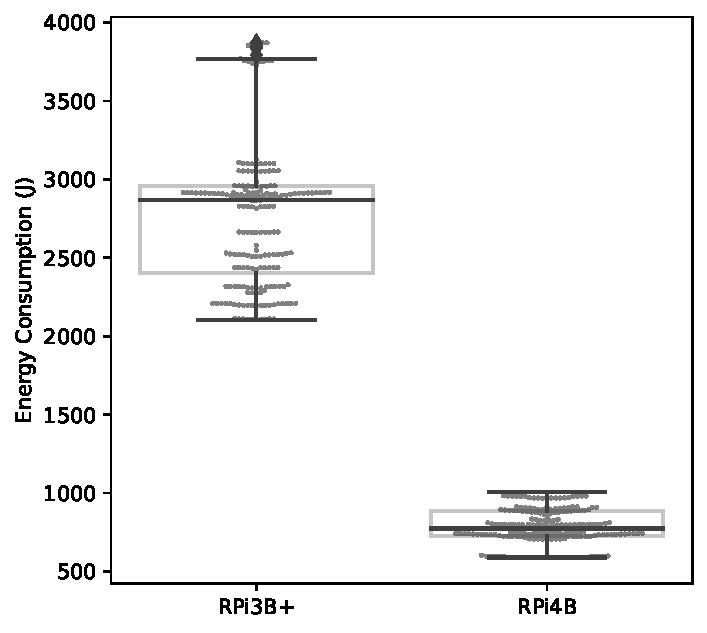
\includegraphics[width=\textwidth]{images/E_per_SUT.pdf}
    \caption{.}
    \label{fig:e_per_sut}
\end{subfigure}
\hspace{\fill}
\begin{subfigure}[t]{0.49\textwidth}
    \centering
    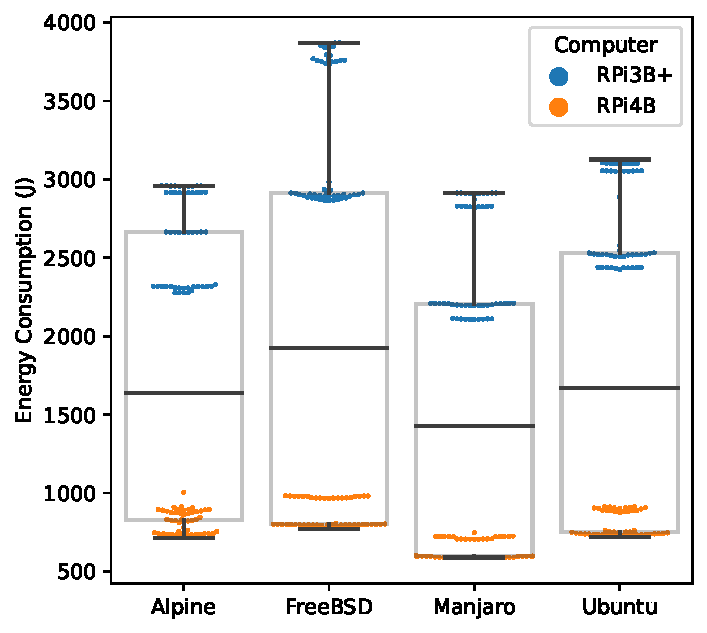
\includegraphics[width=\textwidth]{images/E_per_OS.pdf}
    \caption{.}
    \label{fig:e_per_os}
\end{subfigure}
\hspace{\fill}
\begin{subfigure}{\textwidth}
    \centering
    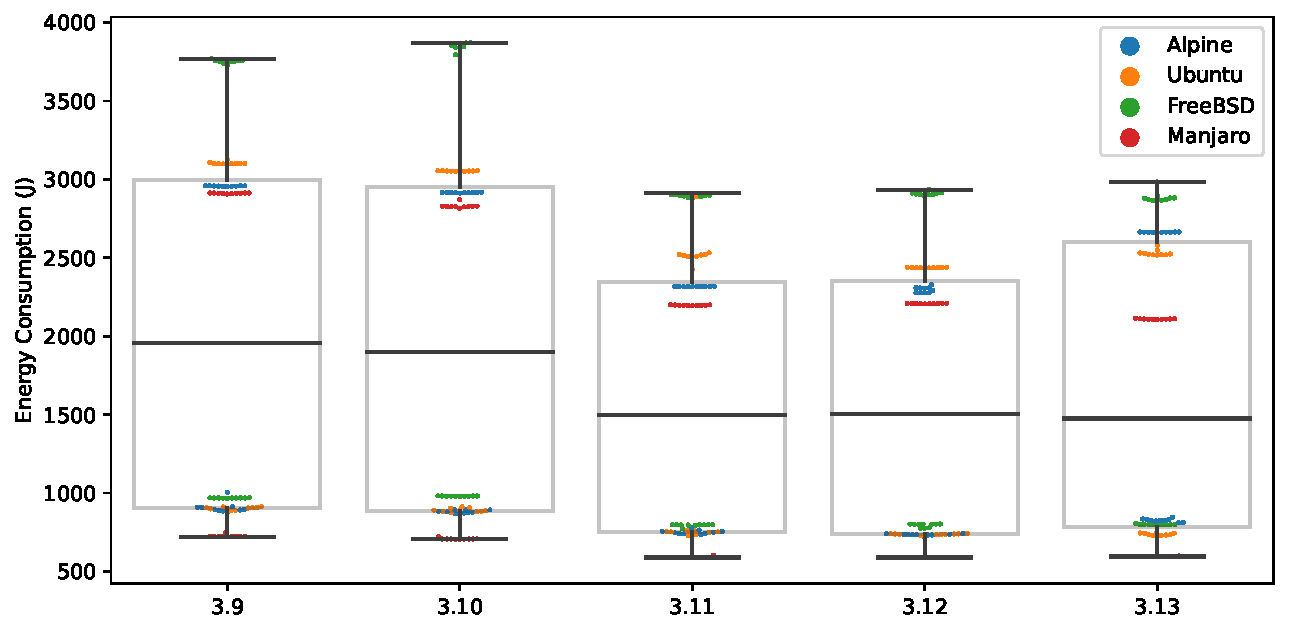
\includegraphics[width=0.9\textwidth]{images/E_per_Python_version.pdf}
    \caption{.}
    \label{fig:e_per_os}
\end{subfigure}
\caption{}\label{fig:e_results}
\end{figure}
\todo{Color dots according to other two features that are not present}



% \begin{figure}[H]
%     \centering
%     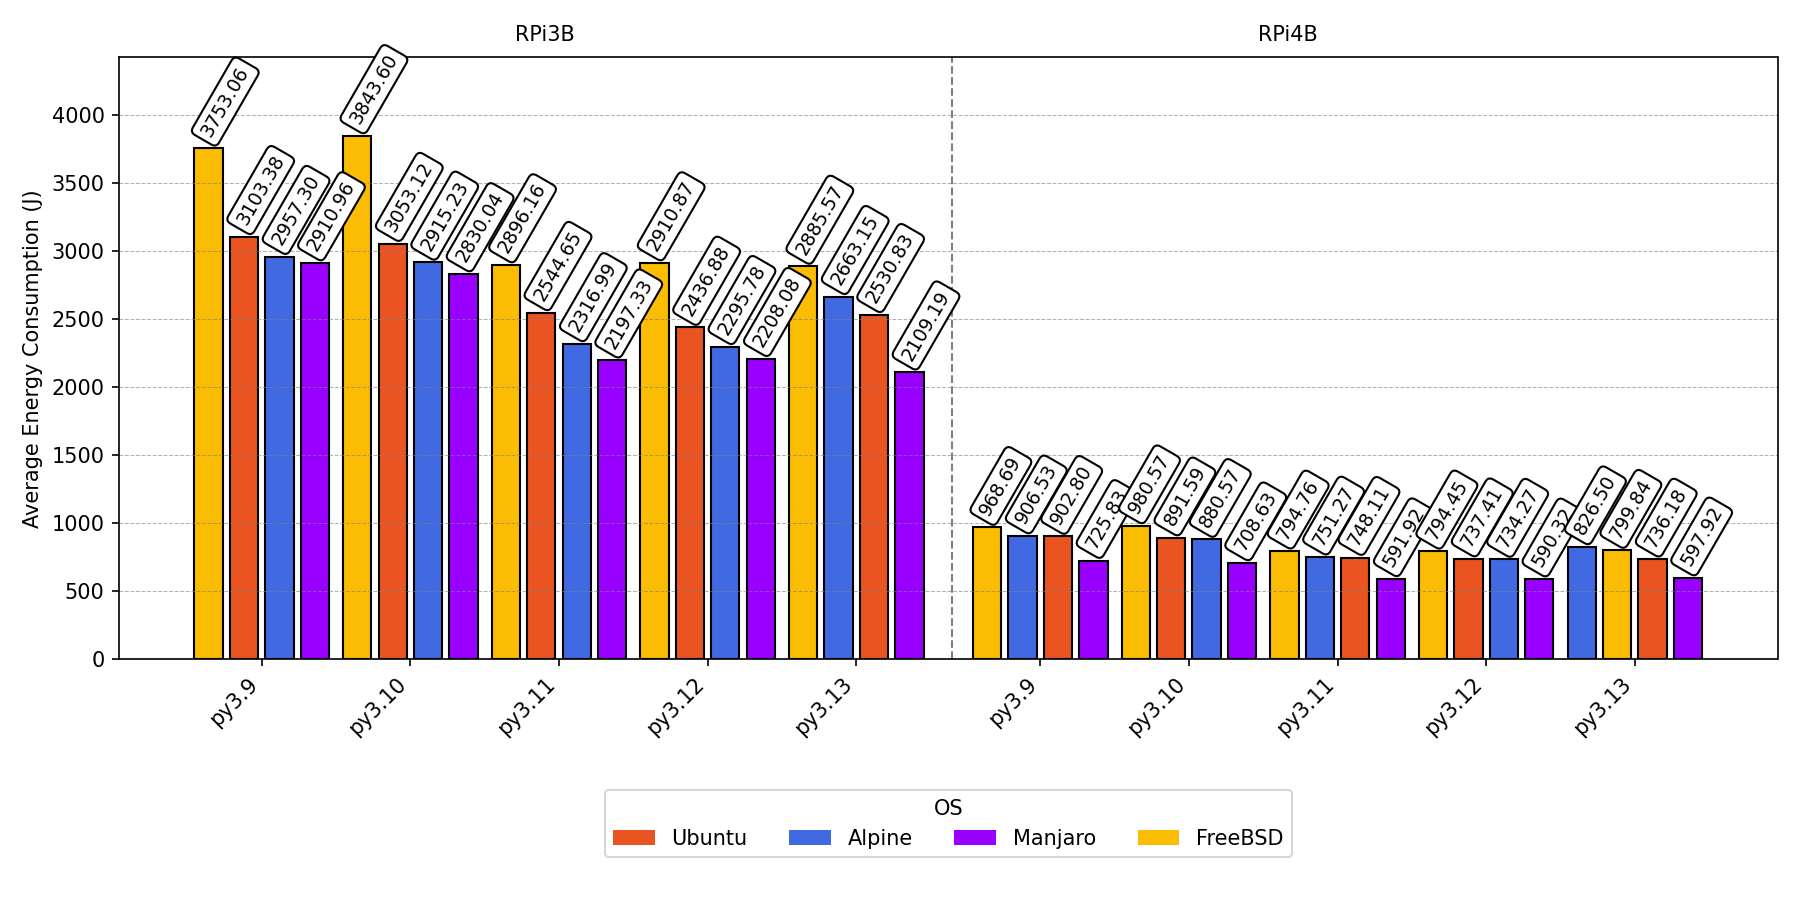
\includegraphics[width=\textwidth]{figures/consumption_barplot_all_pis.png}
%     \caption{Barplot showing the average energy consumption across the 10 recordings made for each configuration.}
%     \label{fig:barplot}
% \end{figure}

% \autoref{fig:barplot} shows the average energy consumption of all benchmarked configurations. The average energy consumption is reflected in both the height of the given column and the label displayed above it. OSs are displayed grouped by Python versions, ordered from lowest to highest version left to right. Within Python version groupings, the OSs are ordered from highest to lowest average energy consumption from left to right. This figure visually indicates, like observed above, RPi3B+ on FreeBSD running Python3.10 having the highest average energy consumption and RPi4B on Manjaro running Python3.12 having the lowest. The figure also clearly indicates a large difference in average energy consumption between the RPi3B+ and RPi4B. A hierarchy between OSs also presents itself, with FreeBSD consistently having the highest energy consumption within a given group (except for Python3.13 on the RPi4B) and Manjaro consistently having the lowest. The hierarchy between Python versions is less clear, but there does seem to be a trend of the higher version having the lower average energy consumption.

% \begin{figure}[H]
%     \centering
%     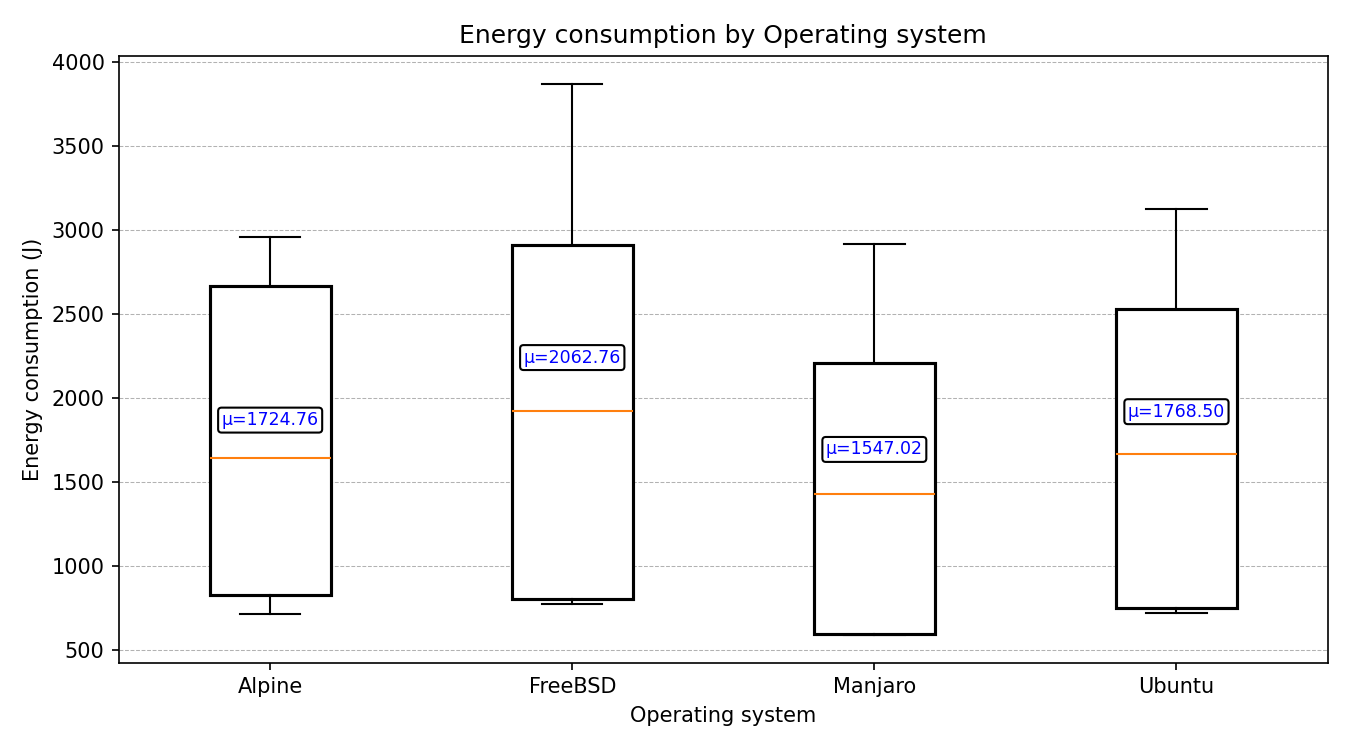
\includegraphics[width=\textwidth]{figures/energy_boxplot_by_os.png}
%     \caption{Boxplot showing the energy consumption of operating systems across all hardware setups and Python versions.}
%     \label{fig:boxplot_os}
% \end{figure}

% \autoref{fig:boxplot_os} shows the energy consumption statistics of OSs across all Python and RPi versions. The minimum is shown by the bottom black line under the white box, the 25th quartile by the bottom of the white box, the median by the orange line, the 75th quartile by the top of the white box, the maximum by the top black bar above the white box and the average ($\mu$) written in blue. These values are extracted from all recordings made for the given OS, such that each box therefore represents 100 individual recordings across 10 configurations. Here we see again a hierarchy of energy consumption, with FreeBSD being highest and Manjaro lowest. We also see an indication that outliers among groups are skewed towards high energy consumption, with the maximum being far removed from the 75th and 25th quartiles. This pattern also indicates that our data for OSs is not normally distributed, but skewed towards the lower end of energy consumption.

% \begin{figure}[H]
%     \centering
%     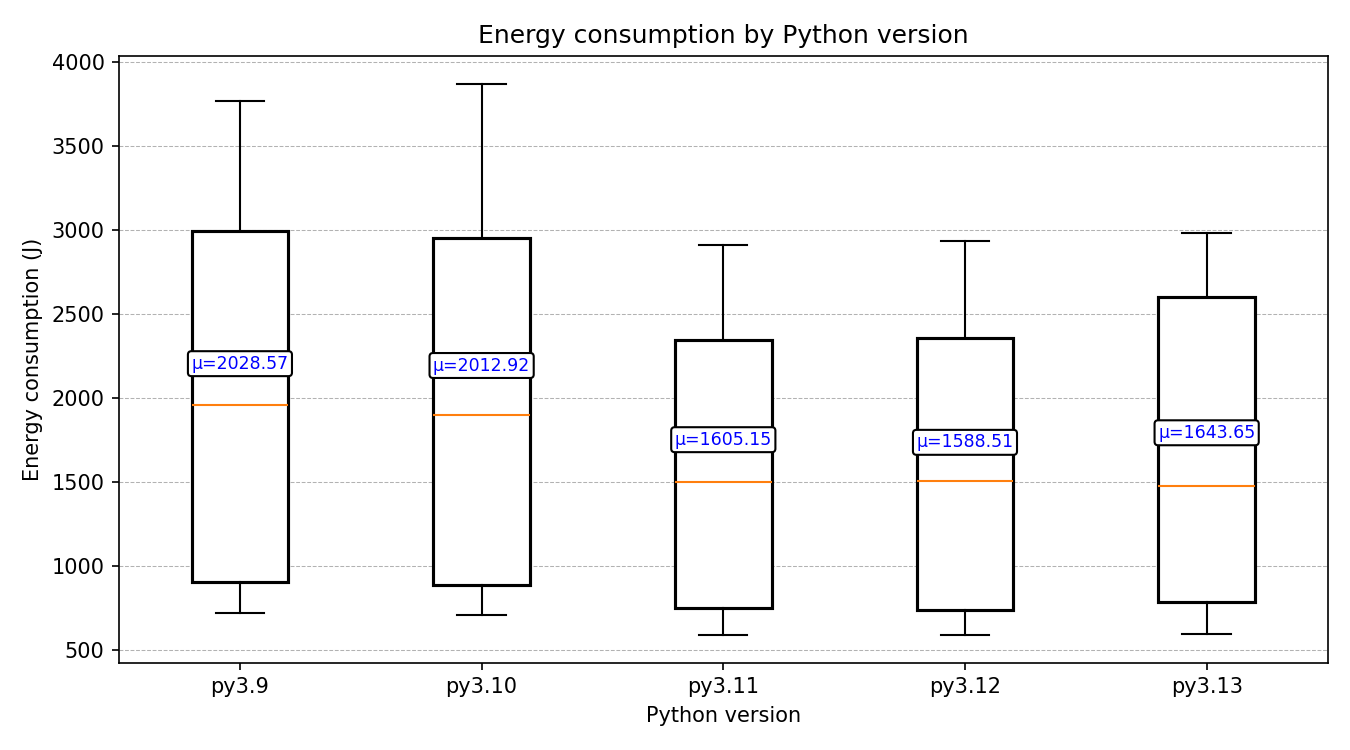
\includegraphics[width=\textwidth]{figures/energy_boxplot_by_python.png}
%     \caption{Boxplot showing the energy consumption of Python versions across all hardware setups and operating systems.}
%     \label{fig:boxplot_python}
% \end{figure}

% \autoref{fig:boxplot_python} shows the energy consumption statistics of Python versions across all operating systems and RPi versions in the same way \autoref{fig:boxplot_os} did for operating systems. These values are accordingly extracted from all recordings made for the Python version, such that each box represents 80 individual recordings across 8 configurations. The hierarchy between Python versions is less clear, but there seems to be a clear decrease in energy consumption from Python3.11 onwards. This data also seems to be skewed towards lower energy consumption, but not as heavily as for OSs. Interestingly, while the values for Python3.11 and 3.12 seem almost equal, the values for Python3.13 seem to be shifted slightly upward, indicating higher energy consumption relative to versions 3.11 and 3.12.

% \begin{figure}[H]
%     \centering
%     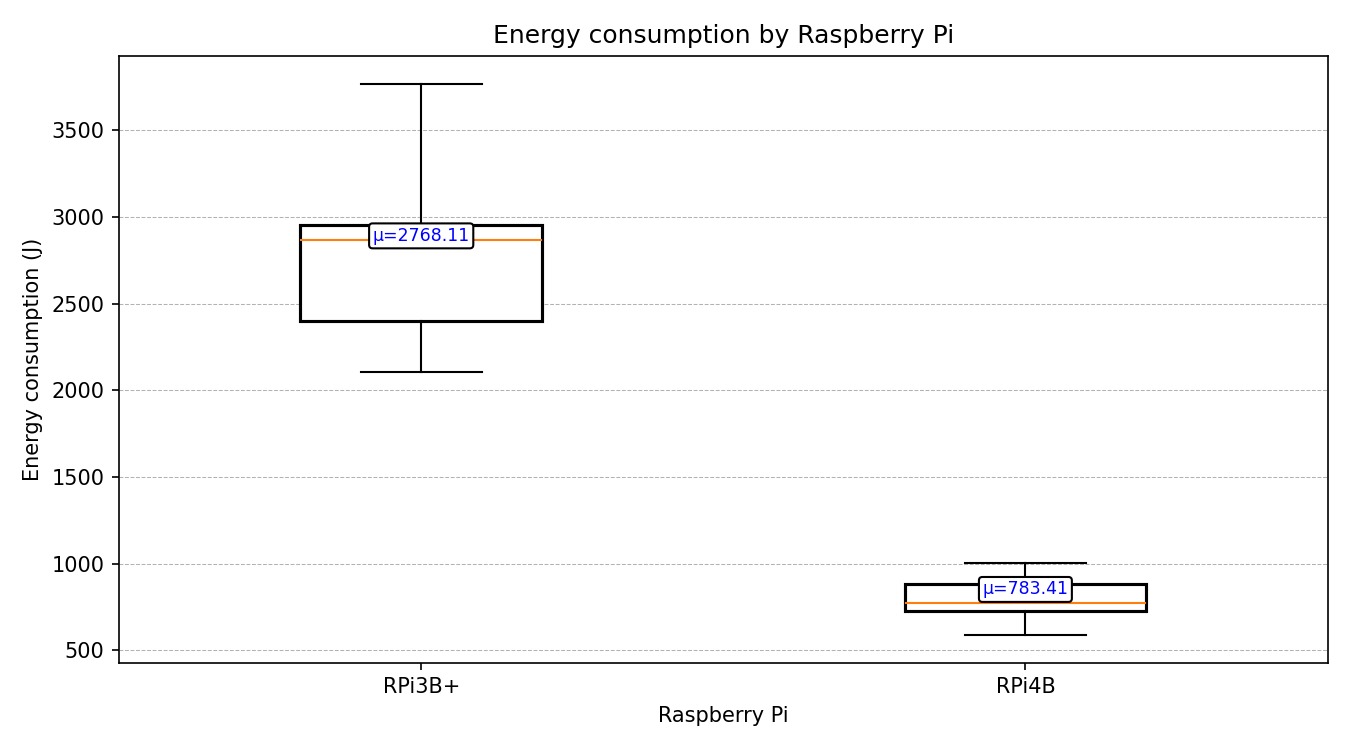
\includegraphics[width=\textwidth]{figures/energy_boxplot_by_rpi.png}
%     \caption{Boxplot showing the energy consumption of RPi versions across all OSs and Python versions.}
%     \label{fig:boxplot_rpi}
% \end{figure}

% \autoref{fig:boxplot_rpi} shows the same statistics as \autoref{fig:boxplot_os} and \autoref{fig:boxplot_python} for the two RPi versions. Each box therefore represents values extracted from 200 individual recordings across 20 configurations. The hierarchy between the two RPis here is readily apparent, with the RPi3B+ having higher energy consumption across the board. The RPi3B+ at first glance seems to have a much higher spread of values, but with recordings ranging from 2000J to well above 3500J compared to a range of just above 500J to around 1000J for the RPi4B, both RPis see just under a doubling in energy consumption from lowest to highest. Both RPis also display a quite balanced range, with only the RPi3B+ being slightly skewed towards lower energy consumption.



\bibliographystyle{splncs04}
\bibliography{bibliography}
%



\end{document}
